

\documentclass{article}
\usepackage{graphicx,amsmath,mdframed}


\newmdtheoremenv{law}{Law}

\title{Computation \& Robot Vision: Lecture 1}
\author{Sam Barrett}

\begin{document}
\maketitle

\section{Camera and image formation}
\label{sec:cif}

\subsection{The human eye}
\label{subsec:human-eye}

The ultimate goal of Computer vision is to allow computers to \textit{see} in a similar (or better) way to humans.

We must first start with what we are trying to emulate: the human eye.

\begin{figure}[ht]
  \centering
  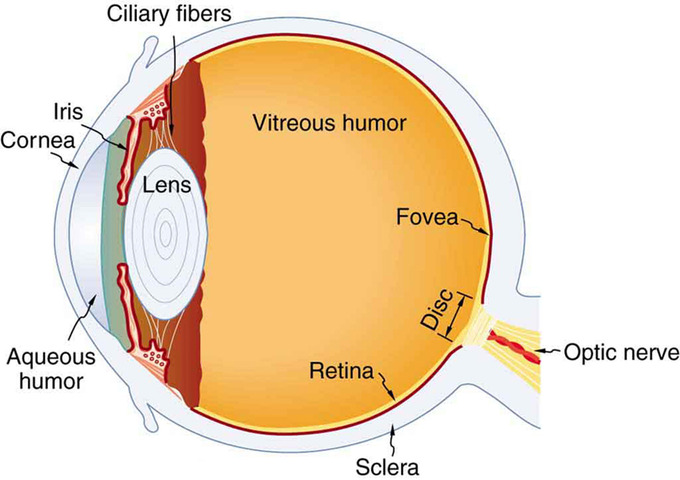
\includegraphics[scale=0.5]{figures/human-eye.jpeg}
  \caption{\label{fig:human-eye} Diagram of the human eye}
\end{figure}

The human eye works by focusing the light entering via the pupil using the lens. This forms an image on the retina.

The retina is made up of many different types of cells, ultimately terminating in the ganglion cells which feed information to the brain via optic nerve fibres. It's composition can be seen in Figure~\ref{fig:retina}.

\begin{figure}[ht]
  \centering
  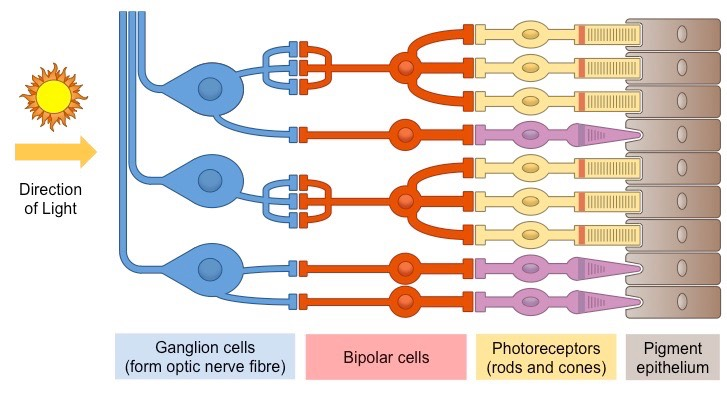
\includegraphics[scale=0.3]{figures/retina_med.jpeg}
  \caption{\label{fig:retina} Diagram of the retina}
\end{figure}

The ganglion cells collect information regarding the visual world from bipolar and amacrine cells. The information takes the form of chemicals messages emitted by receptors on the ganglion cell's membrane.

\subsection{Evolution of cameras}

The evolution of artificial cameras started in the renaissance with the likes of Da Vinci experimenting with camerae obscurae (pinhole image projections) and perspective. Later, photographic film was invented, allowing for the capture of images by exposing the film to different levels of light, focused by a lens the same as we have seen in Figure~\ref{fig:human-eye}.

We have since gone on to develop entirely digital cameras but the principals remain the same. Here, the photographic film containing photosensitive particles is replaced with a camera \textit{sensor} which are arrays of light-sensitive diodes which convert photons to electrons.

\begin{figure}[ht]
  \centering
  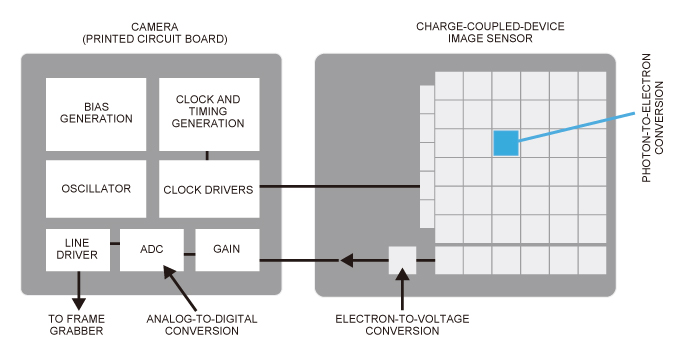
\includegraphics[scale=0.3]{figures/digital-sensor.jpg}
  \caption{\label{fig:digital-sensor} Basic photo-sensor construction }
\end{figure}

Digital images are a 2D grid (or matrix) of integers which show the continuous fluctuations in levels of light.

\subsubsection{Encoding colour}

How do we encode colour into this matrix of integers? We first need to decide on a representation of colour that a computer can understand. We do this by decomposing colours into their primary components. I.e. the different levels of red, green and blue. We can represent \textbf{any} colour using weighted combinations of these colours.

Unfortunately, each photo-diode is \textit{colour blind} and cannot tell the colour of the light hitting it, only it's intensity. So in order to detect the colour of an image, sensors deploy filters such as the Bayer filter. These are layouts of photo-diodes such that each receptor site is known to only detect light from a particular part of the spectrum. The Bayer filter can be seen in Figure~\ref{fig:bayer1}. Using such a filter we can estimate the RGB at each cell using the values of it's neighbours.

\begin{figure}[ht]
  \centering
  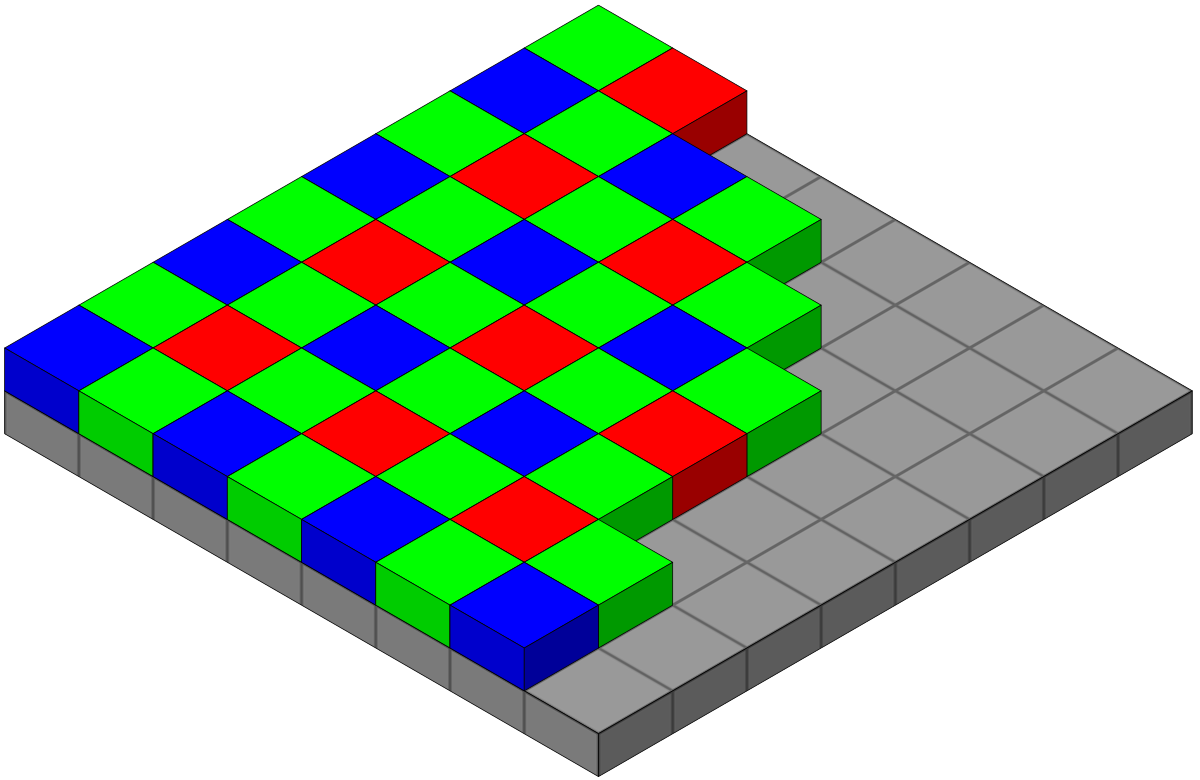
\includegraphics[scale=0.1]{figures/bayer1.png}
  \caption{\label{fig:bayer1} Bayer filter over-top of a sensor}
\end{figure}

\begin{figure}[ht]
  \centering
  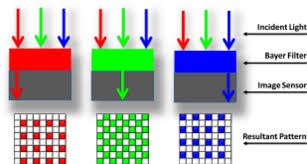
\includegraphics[scale=0.5]{figures/bayer2.jpeg}
  \caption{\label{fig:bayer2} Diagram showing effect of the Bayer filter}
\end{figure}

\textit{Why are there twice as many green as red and blue pixels?}

This is done to mimic the higher sensitivity the human eye has towards green light.

\subsubsection{Digital colour images}

A digital colour image is composed of 3 colour channels. Each channel is a $n\times n$ matrix of intensities representing the intensity of either red, green or blue light at any given position.

We represent each intensity value using an unsigned 8-bit integer (\texttt{uint8}). Using this encoding $(0,0,0)$ represents black and $(255,255,255)$ represents pure white.


\subsection{Pinhole cameras}
\label{subsec:pinhole}

A pinhole camera is an abstract camera model used to explain the principals of modern cameras. They do \textit{work} in practice.

\begin{figure}[ht]
  \centering
  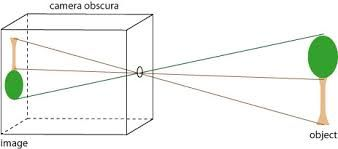
\includegraphics[scale=0.4]{figures/pinholecamera.jpg}
  \caption{\label{fig:pinhole-camera} An example of a pinhole camera}
\end{figure}

There are several notable effects caused by using this perspective projection:

\begin{itemize}
  \item it produces an \textbf{inverted} image.
  \item the size of an object is related to it's distance from the camera.

        In fact, the projections of any 2 parallel lines lying in the same plane, $\Pi$ appear to converge on a horizon line $H$ which lies at the intersection of the image plane with the plane \textbf{parallel} to $\Pi$ passing through the pinhole. This can be observed in real life such as in Figure~\ref{fig:converging-lines}

\end{itemize}



\begin{figure}[ht]
  \centering
  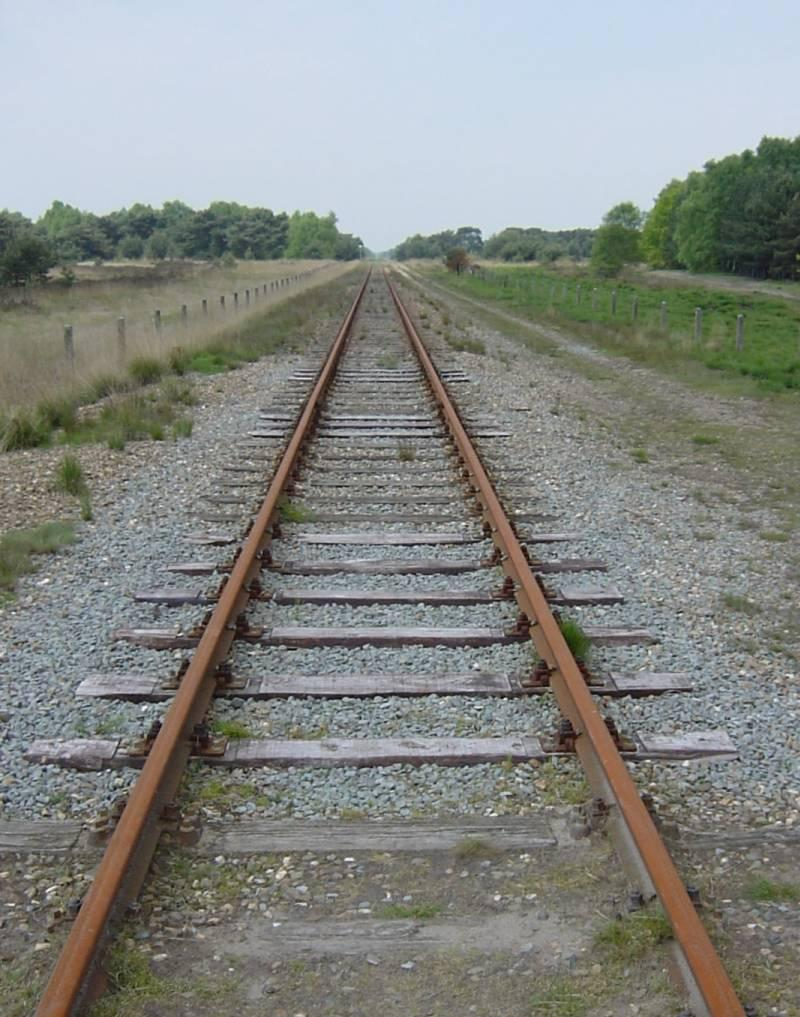
\includegraphics[scale=0.2]{figures/converge.jpg}
  \caption{\label{fig:converging-lines} Two parallel lines appearing to converge on the horizon}
\end{figure}

This effect is captured by our cameras meaning:

\begin{enumerate}
  \item Parallel lines in 3D meet at the same \textit{vanishing point} in the image.
  \item The 3D ray passing through the camera centre and the vanishing point is parallel to the lines.
  \item There (can) exist multiple vanishing points in the camera plane.

        We say the line connecting multiple vanishing points is the horizon line.
\end{enumerate}

These properties can be proved in a geometric fashion, but it is more convenient to reason instead in terms of reference frames, coordinate and equations.

\subsection{The equation of projection}

Consider a coordinate system $(O,\mathbf{i}, \mathbf{j} , \mathbf{k} )$ is attached to the pinhole camera, whose origin $O$ coincides with the pinhole and the vectors $\mathbf{i} $ and $\mathbf{j} $ form a basis for a vector plane parallel to the image plane $\Pi$. $\Pi$ is located a distance $d$ from the pinhole along vector $\mathbf{k}$. The line perpendicular to $\Pi $ and passing through the pinhole is called the optical axis, and the point $c$ where it \textit{pierces} $\Pi$ is called the \textit{image centre}. This point can be used as the origin of an image plane coordinate frame, and is important in camera calibration procedures.

Let $P$ denote a scene point with coordinates (X,Y,Z) and $p$ denote the corresponding image with coordinates $(x,y,z)$
\begin{itemize}
  \item Since $p$ lies on the image plane, we know that $z=d$.
  \item Since the three points $P,O$ and $p$ are co-linear, we know $\vec{Op} = \lambda \vec{OP}$ for some value $\lambda$ so,
        \[
        \begin{cases}
          x = \lambda X \\
          y = \lambda Y & \Longleftrightarrow \lambda = \frac{x}{X} = \frac{y}{Y} = \frac{d}{Z}, \\
          d = \lambda Z
        \end{cases}
        \]

        and therefore, by similar triangles

        \[
        \begin{cases}
          x = d \frac{X}{Z}, \\
          y = d \frac{Y}{Z}
        \end{cases}
        \]

        Where we ignore the third coordinate
\end{itemize}
\textbf{not really sure I follow this in the book or the slides }



\begin{figure}[ht]
  \centering
  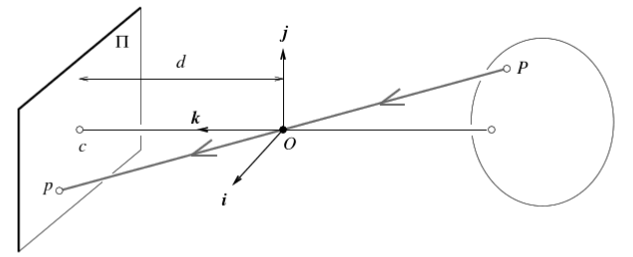
\includegraphics[scale=0.6]{figures/perspectiveproof.png}
  \caption{\label{fig:perspective-proof} Deriving the perspective projection equations }
\end{figure}

\subsection{Weak Perspective}

The pinhole perspective is only an approximation of the geometry of the imaging process. A more accurate model is called \textit{weak} perspective.

Consider the \textit{fronto-parallel} plane $\Pi_{0}$ defined by $Z = Z_{0}$, for any point $P$ in $\Pi_{0}$ we can reformat our earlier equation to form:

\[
  \begin{cases}
    x = -mX, \\
    y = -mY
  \end{cases}
\]

 $ \text{where } m = - \frac{d}{Z_{0}}$

 Physical constrains mean that $Z_{0}$ must be negative (or simply, the plane must be in front of the pinhole), so the magnification $m$ associated with the plane $\Pi_{0}$ is positive.

Consider two points $P$ and $Q$ in $\Pi_{0}$ and their corresponding projected images $p$ and $q$, it is obvious that $\vec{PQ}$ and $\vec{pq}$ are parallel, meaning that $\|\vec{pq}\| = m \| \vec{PQ} \|$. This  simply demonstrates the dependence of image size on object distance that we observed earlier.

An advantage of weak perspective is that it is relatively easy to use but it isn't particularly accurate. It can be used when the scene depth is small relative to the average distance from the camera, i.e. $m$ can be taken to be constant.

\begin{figure}[ht]
  \centering
  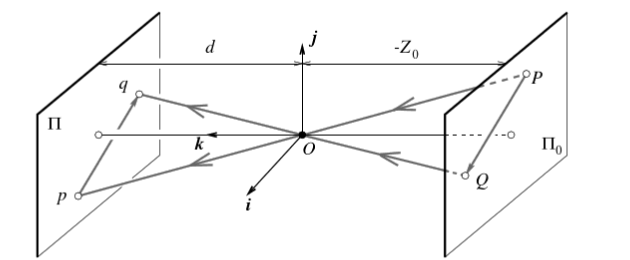
\includegraphics[scale=0.6]{figures/weakperspective.png}
  \caption{\label{fig:weakperspective} Weak Perspective Projection}
\end{figure}


\subsection{Orthographic Projection}

When it is known that the camera always remains at a roughly constant distance from the scene, we can normalise the image coordinates so that $m=-1$. This is the \textit{orthographic projection} and is defined by:

\[
  \begin{cases}
    x = X, \\
    y = Y
  \end{cases}
\]

with all light rays parallel to the $\mathbf{k} $ axis and orthogonal to the image plane $\pi$. This can be an acceptable model in many conditions but the assumption of pure orthographic projection is usually unrealistic.

\begin{figure}[ht]
  \centering
  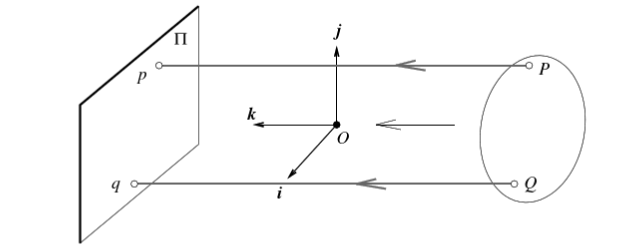
\includegraphics[scale=0.6]{figures/orthperspective.png}
  \caption{\label{fig:orthperspective} Orthographic Projection}
\end{figure}

\subsubsection{Size of pinhole}

\begin{itemize}
  \item Pinhole too big

        Many directions are averaged, blurring the image

  \item Pinhole correctly sized

        Dark but sharp image

  \item Pinhole too small

        Diffraction effects blur the image.
\end{itemize}

Generally, pinhole cameras produce dark images as very little light is allowed through the pinhole onto the sensor.

\subsection{Cameras with lenses}

Most cameras are equipped with lenses, this is to circumvent the issues that arise from using a pinhole.

\begin{itemize}
  \item lenses can help to gather more light
  \item lenses can help to keep the produced image in sharp focus.
\end{itemize}

\subsubsection{The law of geometric optics}

Lenses are governed by the law of geometric optics.

\begin{itemize}
  \item Light travels in straight lines when travelling in homogeneous media.
  \item When a ray is reflected from a surface, this ray, its reflection, and the surface normal are co-planar and the angles between them are complimentary
        \item When a ray passes from one medium to another, it is \textit{refracted}, meaning its direction changes.
\end{itemize}



\begin{law}(Snell's law)
\[
  n_{1}\sin \alpha_{1} = n_{2}\sin \alpha_{2}
\]

Where:

\begin{itemize}
  \item $r_{1}$ is the incident ray
  \item $n_{1}$ and $n_{2}$ are the refractive indexes of the origin medium and destination medium respectively.
  \item $r_{2}$ is the refracted ray
  \item $r_{1}$ and $r_{2}$ are the normal to the incident surface and are co-planar
  \item $\alpha _{1}$ and $\alpha _{2}$ are the angles between the normal and the $r_{1}$ and $r_{2}$
\end{itemize}
\end{law}

When the angles between these rays and the refracting surfaces of the lens are assumed to be small, Snell's law becomes $n_{1}\alpha_{1} \approx n_{2}\alpha_{2}$. \textbf{This is known as the paraxial form of Snell's law.}

If we consider a \textit{thin} lens with two spherical surfaces of radius $R$ and a refractive index of $n$ and we assume the lens is surrounded by a vacuum, rays passing through $O$ are not refracted. This is the case as any ray passing through the right boundary of our lens is refracted but is then refracted precisely the same amount the other way when passing the left boundary.

Consider a point $P$ which is located at $-Z$ from the optical axis (the plane on which the lens sits), and denote a ray $PO$ which passes from this point through the centre of the lens $O$. It follows from our paraxial form of Snell's law that $PO$ is \textbf{not} refracted. It is also the case that all other rays passing through $P$ are focused by our lens to the point $p$ located at a depth of $z$ such that,

\[
  \frac{1}{z} - \frac{1}{Z} = \frac{1}{f}
\]

Where $f= \frac{R}{2(n-1)}$ and is the focal length of the lens.

All of this however, relies on an idealised \textit{thin} lens. In actuality, our lenses do not have these same characteristics.


There are other such aberrations:

\begin{itemize}
  \item Chromatic aberration
        \begin{itemize}
          \item   Light at different wavelengths follows different paths, meaning some wavelengths are defocussed
                \item This can be avoided in machines by coating the lens. Humans cannot avoid it.
        \end{itemize}
  \item Scattering at the lens surface

        \begin{itemize}
          \item Some light entering the lens system is reflected iff each surface it encounters (see Fresnel's law)
          \item This can be circumvented in machines by coating the lens and its interior. Humans must live with it.
        \end{itemize}
\end{itemize}

These aberrations can also be avoided through the use of compound lenses.



\end{document}

